\documentclass{article}
\usepackage{graphicx}
\usepackage{amsmath}
\title{Report 2}
\author{Emerson Schryver}
\begin{document}
\maketitle
\section{Introduction}
\textbf{"Blockbusting" in the 21st Century?: Minority Move-ins and Neighborhood Home Value Appreciation}
I am investigating the extent to which an increase in the minority move-in share of an area modifies future home-value appreciaiton. I am using federal home-loan-level underwriting data (Fannie Mae and Freddie Mac) to track move-ins, Census (ACS) data to normalize, and Zillow ZHVI data to track home prices. My outcome variable is home-value appreciation (normalized to MSA), and my main variable of interest is change in minority move-in share (from the initial period to the "treatment" period) for a given ZIP code. 
% I am also controlling for the initial minority move-in share, the initial move-in share, the terminal minority move-in share, the terminal move-in share, and the MSA average home-value appreciation. I am using a fixed-effects model to control for ZIP code fixed effects. I am also using a two-stage least squares model to control for endogeneity. I am using a 2010-2017 panel dataset with 7732 observations. I am using a 5\% significance level. 
\section{Maps}
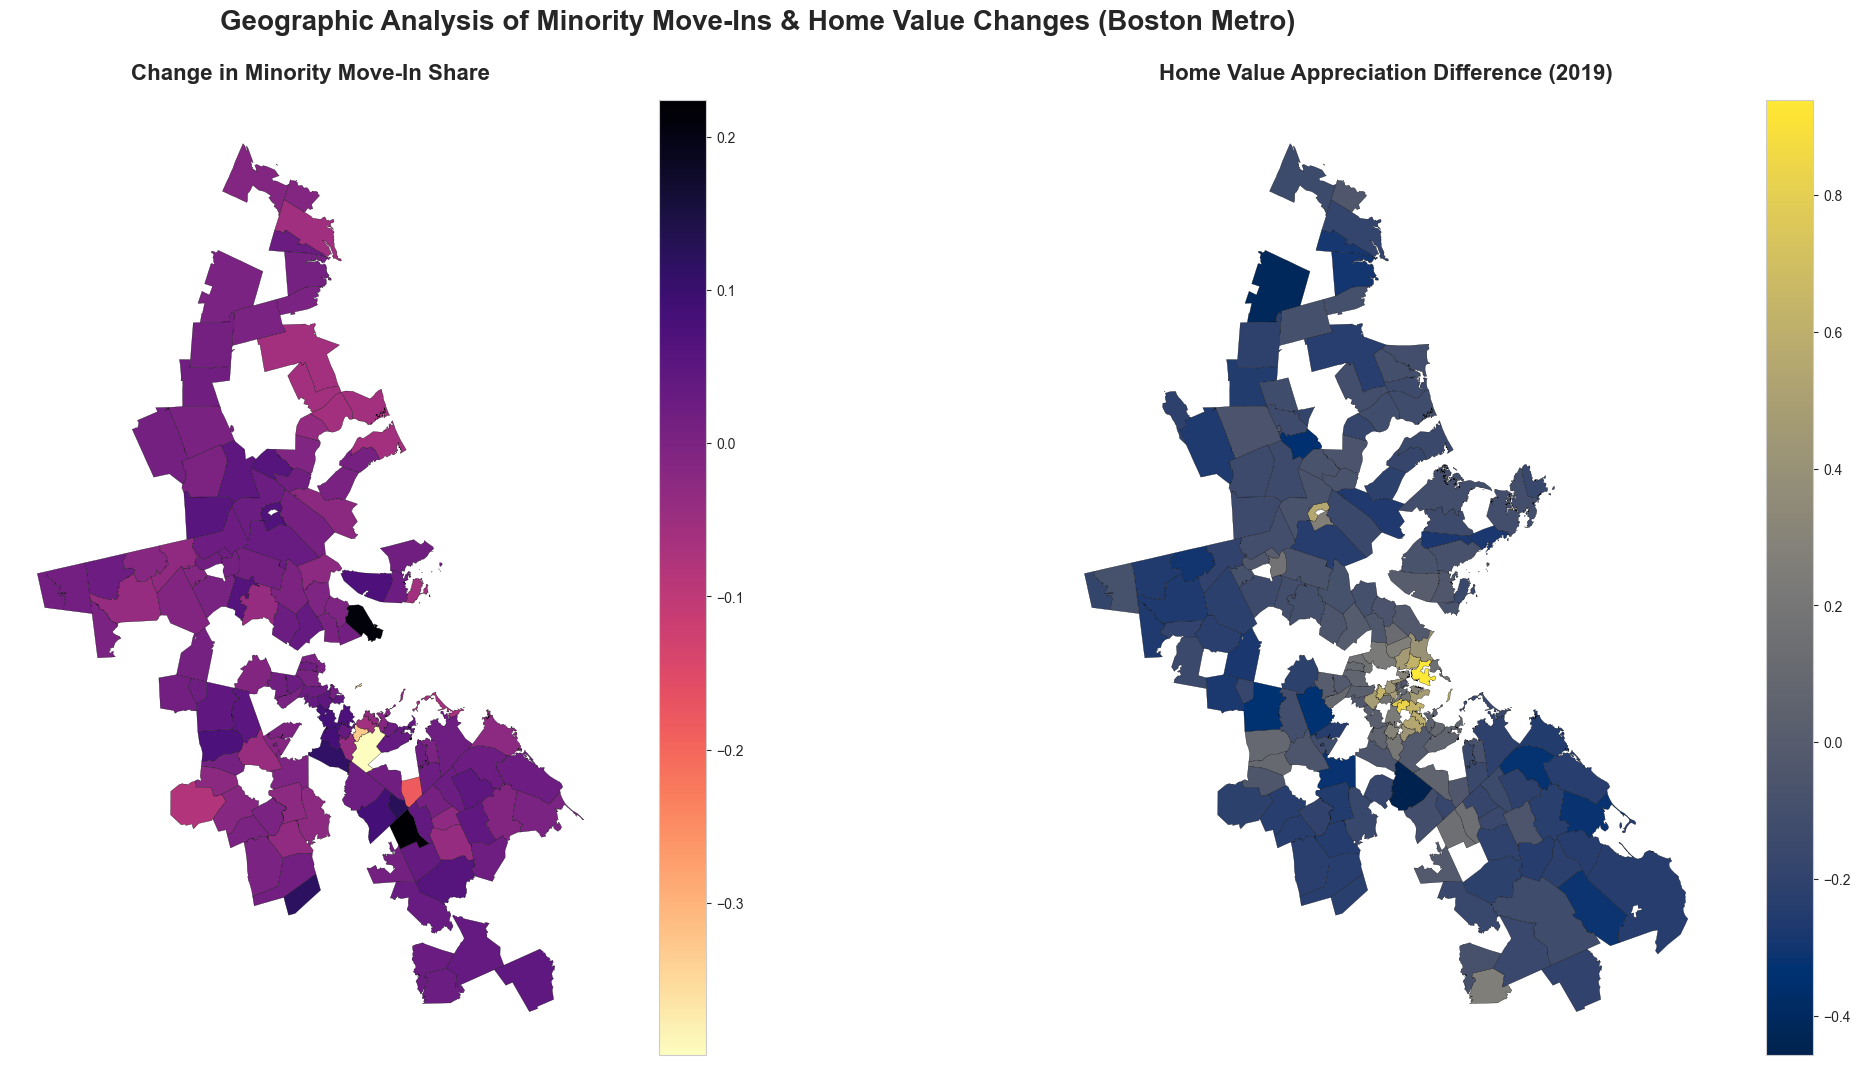
\includegraphics[width=\textwidth]{map.png}

Both of these maps focus on Boston, a particular metro area that is good for analysis (lots of zip codes, a good chunk of single-family neighborhoods). The left map shows my main dependent variable, the change in minority move-in share. The right map shows my main y-variable, the home-value appreication relative to the rest of the MSA. The maps are relatively scattered, and there is no clear obvious correlation, which supports my conclusion that the relationship between minority move-ins and home-value appreciation is unclear.
\section{Regressions}
\begin{table}[!htbp] \centering
\begin{tabular}{@{\extracolsep{5pt}}lcccc}
    \\[-1.8ex]\hline
    \hline \\[-1.8ex]
    & \multicolumn{4}{c}{\textit{Dependent variable: value\_ratio\_2017}} \\
    \cr \cline{2-5}
    \\[-1.8ex] & \multicolumn{4}{c}{Home Value Change (\%) (2010-2017)}  \\
    \\[-1.8ex] & (1) & (2) & (3) & (4) \\
    \hline \\[-1.8ex]
     $\frac{\text{Ratio (T)}}{\text{Ratio (I)}}$ & 0.075$^{***}$ & 0.032$^{**}$ & & \\
    & (0.026) & (0.015) & & \\
     MMI (I) & & & 0.003$^{***}$ & \\
    & & & (0.000) & \\
     $\frac{\text{MMI(I)}}{\text{MI(I)}}$ & & & & 0.030$^{**}$ \\
    & & & & (0.015) \\
     MI (I) & & & -0.000$^{***}$ & \\
    & & & (0.000) & \\
     MMI(T) & & & 0.000$^{}$ & \\
    & & & (0.000) & \\
     $\frac{\text{MMI(T)}}{\text{MI(T)}}$ & & & & 0.180$^{***}$ \\
    & & & & (0.017) \\
     MI(T) & & & -0.000$^{***}$ & \\
    & & & (0.000) & \\
     MSA avg & & 0.806$^{***}$ & 0.801$^{***}$ & 0.777$^{***}$ \\
    & & (0.007) & (0.007) & (0.007) \\
    intercept & 1.336$^{***}$ & 0.133$^{***}$ & 0.156$^{***}$ & 0.151$^{***}$ \\
    & (0.003) & (0.010) & (0.010) & (0.010) \\
    \hline \\[-1.8ex]
     Observations & 7732 & 7732 & 7732 & 7732 \\
     $R^2$ & 0.001 & 0.664 & 0.674 & 0.678 \\
     Adjusted $R^2$ & 0.001 & 0.664 & 0.674 & 0.678 \\
     Residual Std. Error & 0.302 (df=7730) & 0.175 (df=7729) & 0.172 (df=7726) & 0.171 (df=7728) \\
    %  F Statistic & 8.445$^{***}$ (df=1; 7730) & 7624.077$^{***}$ (df=2; 7729) & 3195.555$^{***}$ (df=5; 7726) & 5424.707$^{***}$ (df=3; 7728) \\
    \hline
    \hline \\[-1.8ex]
    \textit{Note:} & \multicolumn{4}{r}{$^{*}$p$<$0.1; $^{**}$p$<$0.05; $^{***}$p$<$0.01} \\
    \end{tabular}
\end{table}
\newpage
With the following variable names:

\begin{tabular}{cc}
    Variable & Description \\\hline
    MMI(I) & Minority move-ins (initial period) \\
    MI(I) & Move-ins (initial period) \\
    MMI(T) & Minority move-ins (treatment period) \\
    MI(T) & Move-ins (treatment period) \\
    MSA avg & Metropolitan Statistical Area average home-value appreciation \\
    Ratio (T) & Minority move-in share (treatment period) \\
    Ratio (I) & Minority move-in share (initial period)
\end{tabular}    
These results suggest little correlation between a change in minority move-ins and future home-value appreciation. The coefficents are surprising alone, but after my results from project 1 are unsurprising. My graphs in project 1 suggested there was little-to-no relationship, which is a similar conclusion to this. The only significant variable is the MSA average home-value appreciation, which is expected.

The fact that my $R^2$ is not incredibly high indicates that it may make sense to control for more variables, such as income and neighborhood political affiliation.
\end{document}